\chapter{Results}

\section{Datasets}

- Problem with sequential data sets

\subsection{Rico}

\begin{itemize}
  \item Too less frames.
  \item No transition between apps.
\end{itemize}

\section{Preprocessing Android UI tree data}
\subsection{Filtering privacy invasive details}
\subsection{Normalization, Feature selection}

Dealing with variable length data tf.io.VarLenFeature()

\section{Model}

%- Screen2Words

Multiple approaches

\todo{create graphic for each approach}

AutoEncoder:

\begin{itemize}
  \item Encoder -> Decoder -> LSTM -> Decoder
  \item Encoder -> LSTM -> Decoder
  \item LSTM -> Encoder -> Decoder (AutoEncoder)
\end{itemize}

Decoder can either only decode to x and y or to whole UI tree.

\section{Evaluation}

\begin{figure}[htbp!]
  \centering
  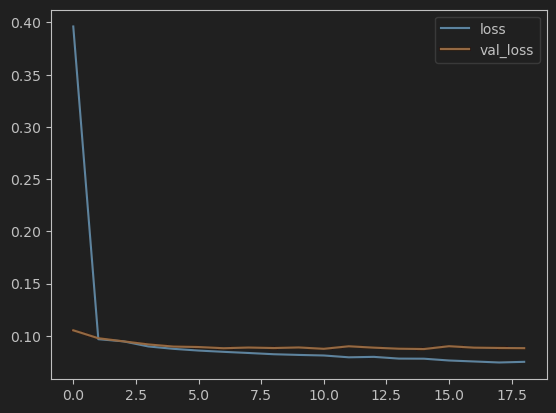
\includegraphics[width=\textwidth]{graphics/model_history_loss}
  \caption{Model loss vs validation loss}
  \label{fig:model_history_loss}
\end{figure}

\subsection{Mean Squared Error}
\subsection{F1 Score}
\section{Limitations}

Dataset
Dataset is not through different apps, only in one app.
Dataset is not detailed enough in the time steps, or not containing all data
Dataset is not long enough
Dataset has no paid apps or apps with login, which most services require
Dataset has wrong data see \cite{clay}

Preprocessing
Need more time to validate what are the core parameters to predict the next user intent


Model needs more investigation on what data is needed
How many neurons are required to achieve this
Play around with different layers, also Convolutional and pretrained embeddings
